% Options for packages loaded elsewhere
\PassOptionsToPackage{unicode}{hyperref}
\PassOptionsToPackage{hyphens}{url}
%
\documentclass[
]{article}
\usepackage{amsmath,amssymb}
\usepackage{lmodern}
\usepackage{iftex}
\ifPDFTeX
  \usepackage[T1]{fontenc}
  \usepackage[utf8]{inputenc}
  \usepackage{textcomp} % provide euro and other symbols
\else % if luatex or xetex
  \usepackage{unicode-math}
  \defaultfontfeatures{Scale=MatchLowercase}
  \defaultfontfeatures[\rmfamily]{Ligatures=TeX,Scale=1}
\fi
% Use upquote if available, for straight quotes in verbatim environments
\IfFileExists{upquote.sty}{\usepackage{upquote}}{}
\IfFileExists{microtype.sty}{% use microtype if available
  \usepackage[]{microtype}
  \UseMicrotypeSet[protrusion]{basicmath} % disable protrusion for tt fonts
}{}
\makeatletter
\@ifundefined{KOMAClassName}{% if non-KOMA class
  \IfFileExists{parskip.sty}{%
    \usepackage{parskip}
  }{% else
    \setlength{\parindent}{0pt}
    \setlength{\parskip}{6pt plus 2pt minus 1pt}}
}{% if KOMA class
  \KOMAoptions{parskip=half}}
\makeatother
\usepackage{xcolor}
\usepackage[margin=1in]{geometry}
\usepackage{longtable,booktabs,array}
\usepackage{calc} % for calculating minipage widths
% Correct order of tables after \paragraph or \subparagraph
\usepackage{etoolbox}
\makeatletter
\patchcmd\longtable{\par}{\if@noskipsec\mbox{}\fi\par}{}{}
\makeatother
% Allow footnotes in longtable head/foot
\IfFileExists{footnotehyper.sty}{\usepackage{footnotehyper}}{\usepackage{footnote}}
\makesavenoteenv{longtable}
\usepackage{graphicx}
\makeatletter
\def\maxwidth{\ifdim\Gin@nat@width>\linewidth\linewidth\else\Gin@nat@width\fi}
\def\maxheight{\ifdim\Gin@nat@height>\textheight\textheight\else\Gin@nat@height\fi}
\makeatother
% Scale images if necessary, so that they will not overflow the page
% margins by default, and it is still possible to overwrite the defaults
% using explicit options in \includegraphics[width, height, ...]{}
\setkeys{Gin}{width=\maxwidth,height=\maxheight,keepaspectratio}
% Set default figure placement to htbp
\makeatletter
\def\fps@figure{htbp}
\makeatother
\setlength{\emergencystretch}{3em} % prevent overfull lines
\providecommand{\tightlist}{%
  \setlength{\itemsep}{0pt}\setlength{\parskip}{0pt}}
\setcounter{secnumdepth}{5}
\usepackage{fancyhdr}
\usepackage{lipsum}
\pagestyle{fancy}
\fancyfoot[CO,C]{© Copyright 2022 Beneficiaries of the EuroCC/Castiel Project}
\fancyfoot[RO]{\thepage}
\ifLuaTeX
  \usepackage{selnolig}  % disable illegal ligatures
\fi
\IfFileExists{bookmark.sty}{\usepackage{bookmark}}{\usepackage{hyperref}}
\IfFileExists{xurl.sty}{\usepackage{xurl}}{} % add URL line breaks if available
\urlstyle{same} % disable monospaced font for URLs
\hypersetup{
  hidelinks,
  pdfcreator={LaTeX via pandoc}}

\author{}
\date{\vspace{-2.5em}}

\begin{document}

\begin{center}

  
\includegraphics[width=0.3\textwidth]{media/image1.jpeg}

  \bigskip \bigskip \bigskip \bigskip \bigskip 

  \LARGE\textbf{Developing Shiny application}

  \bigskip \bigskip \bigskip 

  \LARGE{Best Practice Guide}
  
  \bigskip \bigskip

  \large{October 2022}

  \bigskip \bigskip \bigskip \bigskip \bigskip 

  
\includegraphics[width=0.35\textwidth]{media/image2.png}
  \qquad \qquad
  
\includegraphics[width=0.4\textwidth]{media/image3.png}

  \bigskip \bigskip \bigskip \bigskip \bigskip 

  
\includegraphics[width=0.6\textwidth]{media/image4.png}
\end{center}

\newpage
\tableofcontents
\newpage

\hypertarget{introduction}{%
\section{Introduction}\label{introduction}}

To understand the terms of data analysis, or to learn a specific
programming language (R in this case), can be difficult for many people.
Providing a single user-friendly application containing visualisations
of the results might be very useful. To do so, it is important to put
together requirements for such application. You have to ask yourself (or
your customer), which unit it will be running on (cloud server, user
laptop, mobile, \ldots), how big data sets you will be processing, or
what features or functions you will need, and so on. Keep in mind, that
requirements can change during the time based on the user feedback.
Moreover, it is better to start with a simple application and gradually
add new functionalities rather than plan and implement whole application
at once. Therefore, the recommendation is to implement individual
functions as standalone modules. The modules can then be simply
modified, added, or removed from the application. Further, to obtain
some user feedback on the application, a mock-up design has to be
created. The mock-up design helps you to ensure that the application
satisfies all the specified requirements during the process. It also
helps to check, if there is something missing in the app, if the app is
understandable, or it is easy to work with. You can also realise that
application contains features which are not necessarry for the whole
software, and can be removed.

\hypertarget{developing-process}{%
\section{Developing process}\label{developing-process}}

The developing process can be summarised as follows:

\begin{itemize}
\tightlist
\item
  define requirements for the application,
\item
  create mock-up design,
\item
  select suitable technology (packages, tools),
\item
  create project enviroment (implement R base codes, move the codes to
  the application, use version control, create tests for the
  application, user testing, etc.)
\item
  if everything is all right, deploy the app.
\end{itemize}

With this process at hand, you will be able to deploy the app without
any further problems. If there are some bugs, or the requirements are
updated, just update the design, the codes, and build app again. In the
text below, example of developing a simple ``Shiny app'' is provided.
Also, brief summaries of R packages suitable for building the Shiny app
are contained in the text.

\hypertarget{requirements}{%
\subsection{Requirements}\label{requirements}}

The requirements are integral part of all the softwares and
applications, which are being developed around the world. It is the very
first step to make clear what are your needs. You have to specify the
requirements on the software, or you have to ask your customer about
them, at the very beginning of the development process. For example,
consider the situation, in which you have to create following
application:

\begin{itemize}
\tightlist
\item
  the application has to run either on Windows OS, Linux OS, or macOS,
  i.e.~on notebook or desktop PC (R language is cross-platform!),
\item
  the user will work with own datasets (upload dataset, tidy dataset,
  show dataset, etc.),
\item
  the user will want to plot some dataset summaries,
\item
  the user will need some clustering methods,
\item
  also an authentication to the app will be needed (for restricted
  data).
\end{itemize}

If the list of requirements exists, you can start developing the
application. Since the Shiny serves as extension for R to create
application using R code, it is a good habit to implement funcionalities
at R itself and test them, at first. Then, move these functions, or
modules, into the Shiny app. While moving into the Shiny app, you have
to think about a mock-up design of the application, i.e.~how to put all
the features together and connect them to a user interface.

\hypertarget{mock-up-design}{%
\subsection{Mock-up design}\label{mock-up-design}}

The mock-up design is being created to provide a better idea of the
graphical user iterface. The draft version helps you realise:

\begin{itemize}
\tightlist
\item
  what inputs are needed, and in which format (numeric, character,
  dataframe, \ldots),
\item
  what outputs will be produced, and in which format (numeric,
  character, dataframe, \ldots),
\item
  the need of (interactive) plots/images, if any,
\item
  if the application will be single or multi page,
\item
  etc.
\end{itemize}

You can create the mock-up desing by hand on the paper, use some of the
graphical softwares (designers), or implement basic UI straight into
Shiny (if you are familiar with Shiny). If you have no experiences with
creating mock-up design (the application at all), we recommend you to
use some of the existing designers. You can find plenty of them on the
internet. Just search, e.g., for ``applications mock-up designer''. They
help you imagine how the inputs look like, help you create (responsive)
layouts, and so on. Drawing design by hand can be the fastest way,
especially if you are experienced in mock-up creation, but for a
customer, output of the mock-up designer is probably more suitable.

\hypertarget{package-tool-selection-based-on-mock-ups-and-requirements}{%
\subsection{Package tool selection based on mock-ups and
requirements}\label{package-tool-selection-based-on-mock-ups-and-requirements}}

With the mock-up design and the requirements at hand, you can decide
which package tool, you will use. You can work with package providing
simple predefined template, or you can use packages providing feancy
styling of the app components, etc.

Focusing on the R programming language, which is commonly used for the
data analysis, there are packages for the graphical interface such as
Shiny, BS4Dash, or ShinyMobile in the R universe. These frameworks
provide a set of functions which allow you to create standalone web
applications or embed them into R markdown documents. You can create
application with graphical interface similar to the existing webpages
(webpage applications), or if you are familiar with CSS styling and JS,
there could be no difference! Below, a brief introduction of each is
given.

\hypertarget{shiny}{%
\subsubsection{Shiny}\label{shiny}}

Shiny is an R package that makes it easy to build interactive web apps
straight from R. You can host standalone apps on a webpage or embed them
in R markdown documents or build dashboards. You can also extend your
Shiny apps with CSS themes, htmlwidgets, and JavaScript actions. You do
not need any web development experience at all. Shiny includes built-in
input widgets, which can be easily used with minimal syntax knowledge.

For more information visit \url{https://shiny.rstudio.com/} .

\hypertarget{bs4dash}{%
\subsubsection{BS4Dash}\label{bs4dash}}

BS4Dash package provides an extension for a Shiny package. It relies on
the Bootstrap 4, which is not natively supported by Shiny. BS4Dash
allows you to develop a Shiny app with more professional look and feel.
Some of the main features are fullscreen toggle, popover, tooltips,
right sidebar, dashboard user dropdown, beautiful preloaders, etc.

For more information visit \url{https://rinterface.github.io/bs4Dash/} .

\hypertarget{shinymobile}{%
\subsubsection{ShinyMobile}\label{shinymobile}}

ShinyMobile is built on the top of the latest Framework 7. It supplies
functions to develop an application especially for iOS and Android. In
other words, it includes Shiny widgets adapted for all mobile platforms.
ShinyMobile is PWA capable, meaning that it can be displayed full screen
on many mobile devices.

For more information visit
\url{https://rinterface.github.io/shinyMobile/} .

\hypertarget{shiny-extensions}{%
\subsubsection{Shiny extensions}\label{shiny-extensions}}

There are lots of frameworks for the R distribution, which can be used
to create the application. There is also a gitlab repository containing
structured list of many (not all) Shiny extensions at
\url{https://github.com/nanxstats/awesome-shiny-extensions}. This is a
good starting point to understand what is done in terms of Shiny
development. Of course, you can look for others on the internet
yourself.

\hypertarget{creation-of-the-project-environment}{%
\subsection{Creation of the project
environment}\label{creation-of-the-project-environment}}

The requirements help you to get an idea how complex your application
will be. If the application will be simple, you can already start to
implement the functions, the modules, without any advanced tools.
However, some applications can be really complex. More complex
applications have code readability issues. This can lead to difficult
debugging due to many interconnections between modules, and so on. Also
be aware of interface complexity, i.e.~there are many inputs, or outputs
defined in user interface to make application clearly understandable. To
avoid problems like these, it is a good habit to find a balance between
those two complexities. Think twice about the application before you
start to implement it, but do not worry if it looks scary at first
sight. In the R universe, there exist frameworks, which help you to
manage the whole project from the beginning, starting with the
implementation step all the way to the product deployment, so there will
be less troubles in your development process. One of these frameworks,
the Golem package, is described below.

\hypertarget{golem-package}{%
\subsubsection{Golem package}\label{golem-package}}

\begin{quote}
Golem is a toolkit for simplifying the creation, development, and
deployment of a shiny application.
\end{quote}

Everything about the golem package can be found at
\href{https://engineering-shiny.org/golem.html}{https://engineering-shiny.org/}.
The book also presents the idea of engineering process to develop and
successfully deploy the app. Here is a short introduction of the golem
package as mentioned in the provided book.

If you create a new golem project, in this case it is called golex
(golem example), a structured folder architecture will be created.

\begin{verbatim}
golex
├── DESCRIPTION
├── NAMESPACE
├── R
│   ├── app_config.R
│   ├── app_server.R
│   ├── app_ui.R
│   └── run_app.R
├── dev
│   ├── 01_start.R
│   ├── 02_dev.R
│   ├── 03_deploy.R
│   └── run_dev.R
├── inst
│   ├── app
│   │   └── www
│   │       └── favicon.ico
│   └── golem-config.yml
└── man
    └── run_app.Rd
\end{verbatim}

At the \textbf{DESCRIPTION} file, you will add series of metadata about
the application. The name of the author(s), version of the app, what is
its purpose, etc. It will be filled automatically by running the scripts
from \textbf{\textbackslash dev} folder. The \textbf{NAMESPACE} defines
how to interact with the rest of the package (application) and it will
never be touched by you. This file will be also created in an automated
way when running the documenting process of your R package. All R
functions (all app functions) will be held in \textbf{/R} folder. Each R
file used during development should be stored in \textbf{/dev} folder.
In the \textbf{/inst/app/ww,} you will keep every CSS or JS files which
define the final look of your application. The golem configuration can
be set in \textbf{golem-config.yml} or you can use \textbf{golem\_opts}
in the \textbf{run\_app()} function. The purpose of the last
\textbf{/man} folder is to held package documentation.

As you can see, the golem package really helps you to implement and
successfully deploy the app. It helps you to maintain the package
structure and even build the app. For more ideas to create
production-grade Shiny app, and other information about the golem
package, please visit the link above. You can use another source of
information, of course. There are plenty of them in the internet.

\hypertarget{githubgitlab}{%
\subsubsection{GitHub/GitLab}\label{githubgitlab}}

Successful development of larger applications cannot be possible without
any ``smart'' code archives. If you are creating a complex package, you
can easily make a mistake and you will disrupt the rest of the code. In
that case, you will want to use last functional version of the
application, so you have to archive it from time to time. The better way
is to use a version system like Github, Gitlab, Bitbucket, and so on.
You can upload whole new project, or just changes, fetch new data, etc.
by simple \textbf{git} commands from terminal (command line). It will
check every change from the last files to a new one, so if you make a
mistake, you just use previous version of a file. Moreover, if you do
not like terminal's (command line's) commands, you can use some of the
existing graphical git softwares to manage your git repository or you
can use built-in git system in the RStudio. If the git repository is
initialised within the project folder, you can do all git commands from
RStudio itself. The last option is to use web application of the used
version systems to manage stored files. Most version systems provide
this functionality. It is only up to you, which way is the most suitable
for you.

\hypertarget{tests}{%
\subsection{Tests}\label{tests}}

Before the package is ready to deploy, the tests have to be done. It
automatically checks if the application can be built without any
problems, functions behave as expected, and so on. In general, the tests
can be divided in three sections:

\begin{itemize}
\tightlist
\item
  Unit tests - functions behave as expected,
\item
  Server function tests - testing of reactive components and outputs,
\item
  Snapshot-based tests - simulate user actions, like clicking on the
  buttons, take snapshots of the application state, and compare the app
  state with the saved snapshots.
\end{itemize}

You can for example use \textbf{runTests()} function in Shiny 1.5.0 and
more to test your app. Simple example of application with defined tests
can be created by \textbf{shinyAppTemplate(``app\_name'')} with used
option \textbf{1: All}. It will generate folder structure with
\textbf{/tests}. For more information, see
\url{https://shiny.rstudio.com/articles/testing-overview.html}. Code
tests can be also done with a testthat package, see
\url{https://testthat.r-lib.org/}.

\hypertarget{continuous-integration}{%
\subsubsection{Continuous integration}\label{continuous-integration}}

In short, Continuous Integration (CI) means that multiple developers
push small changes frequently into shared repository. Moreover, after
each push it is important to run automated tests to verify the
integration of a new code into the package (application). Some of the
version systems are CI-friendly. For example Github has a feature Github
Actions to realise CI.

\hypertarget{release}{%
\subsection{Release}\label{release}}

If you try to find \textbf{what is a software release} on the internet,
you can for example find a webpage
\url{https://www.techtarget.com/searchsoftwarequality/definition/release},
in which the release is defined as

\begin{quote}
A release is the distribution of the final version or the newest version
of a
\href{https://www.techtarget.com/searchapparchitecture/definition/software}{software}
application. A software release may be public or private and generally
signifies the unveiling of a new or upgraded version of the application.
\end{quote}

In other words, you can release the application after all implementation
is done and all tests are valid, i.e.~you can deploy the app to the
product.

\hypertarget{building-blocks}{%
\section{Building blocks}\label{building-blocks}}

Some of the possible functionalities of the Shiny will be discussed in
this section. Here you will learn how to create a login screen, which
plot libraries exist, how to use interactive data tables, how to
transfer data, connect your application to a database, and learn about
the difference between R6 and S3 model.

\hypertarget{login-screen}{%
\subsection{Login screen}\label{login-screen}}

You do not need to worry about whether the Shiny is able to provide a
login screen, because it can! To learn how to create a login page, you
can visit
\url{https://towardsdatascience.com/r-shiny-authentication-incl-demo-app-a599b86c54f7}.

The author of the given hands-on tutorial considers 3 approaches to
build the login page:

\begin{enumerate}
\def\labelenumi{\arabic{enumi}.}
\tightlist
\item
  the basics of the authentication is covered,
\item
  the login form and the corresponding server logic is packed into
  seperate modul (as we mention above, using modules within app is
  powerful),
\item
  the use of shinyauthr package is discussed (it also includes password
  hashing).
\end{enumerate}

You can find other tutorials on the internet, e.g.~you can inspire
yourself at \url{https://stackoverflow.com}. The important thing is that
you are able to create the login screen in the Shiny without any
obstacles. It is up to you which method you will use.

\hypertarget{visualisations---plot-libraries}{%
\subsection{Visualisations - plot
libraries}\label{visualisations---plot-libraries}}

The first step to understand the data is to visualise them. The Shiny
provides several methods to do so. You can use static plots, interactive
plots, or you can even display the data on interactive maps using
Leaflet package. Brief summaries for each of them are stated below.

\hypertarget{static}{%
\paragraph{Static}\label{static}}

Usage of the static plots in the Shiny is quite the same as in R itself.
Data can be visualised using for example ggplot2 library. Hovewer, there
is one difference in the Shiny. You have to use \texttt{plotOutput()}
command on the UI side, and \texttt{renderPlot()} on the server side.
Displaying the images is also possible in the Shiny. To render an image,
you will use \texttt{imageOutput()} and \texttt{renderImage()}. Look
into the help to get familiar with these commands.

\hypertarget{interactive}{%
\paragraph{Interactive}\label{interactive}}

Interactive plots within the Shiny app are powerful feature.
\texttt{plotOutput()} defines four different mouse events:

\begin{itemize}
\tightlist
\item
  \textbf{click} for a single mouse click,
\item
  \textbf{dblclick} for a double click,
\item
  \textbf{hover} to do something when mouse stays in the same place
  within the plot for a while,
\item
  \textbf{brush} to use a rectangular selection tool.
\end{itemize}

The examples of the given events can be found
\url{https://mastering-shiny.org/action-graphics.html}.

For some advanced interactive plots, visit
\url{https://shiny.rstudio.com/articles/plot-interaction-advanced.html}.

While creating an interactive plots, you have to keep in mind that it
takes some time to respond to the event. In other words, when you click
into a plot, the application has to register the event, evaluate the
event (do defined operations), and render updated plot. You also have to
take into account a response of the server (transfer speed) if you
deployed the app at the website.

\hypertarget{leaflet}{%
\paragraph{Leaflet}\label{leaflet}}

As it is stated at the website \url{https://rstudio.github.io/leaflet/}.

\begin{quote}
\href{https://leafletjs.com}{Leaflet} is one of the most popular
open-source JavaScript libraries for interactive maps. It's used by
websites ranging from
\href{http://www.nytimes.com/projects/elections/2013/nyc-primary/mayor/map.html}{The
New York Times} and
\href{http://www.washingtonpost.com/sf/local/2013/11/09/washington-a-world-apart/}{The
Washington Post} to
\href{https://github.com/blog/1528-there-s-a-map-for-that}{GitHub} and
\href{https://www.flickr.com/map}{Flickr}, as well as GIS specialists
like \href{http://www.openstreetmap.org/}{OpenStreetMap},
\href{http://www.mapbox.com/}{Mapbox}, and
\href{http://cartodb.com/}{CartoDB}.

This R package makes it easy to integrate and control Leaflet maps in R.
\end{quote}

The Leaflet package provides functions to easily integrate the maps into
the Shiny app. How to use the Leaflet package is described at
\url{https://rstudio.github.io/leaflet/shiny.html}.

\hypertarget{tables}{%
\subsection{Tables}\label{tables}}

There are two ways to display data in tables. A static one and a dynamic
one. It depends whether you need to just display the data or you need to
filter and sort visualised data.

\hypertarget{static-1}{%
\paragraph{Static}\label{static-1}}

Rendering data in the static table is done using \texttt{tableOutput()}
and \texttt{renderTable()}. It will display the data in the given place
of the app. Static table is suitable for displaying small matrices and
data frames.

\hypertarget{interactive-1}{%
\paragraph{Interactive}\label{interactive-1}}

Interactive tables are the best way to represent data frames in the
Shiny app. You can use built-in commands such as
\texttt{dataTableOutput()} and \texttt{renderDataTable()} or use another
package such as \textbf{reactable}, see
\url{https://glin.github.io/reactable/index.html}.

Interactive tables have wide range of utilities like search function,
sort columns, define number of visible rows per page, navigate through
the table's pages, and so on.

\hypertarget{data-transfer-logic}{%
\subsection{Data transfer logic}\label{data-transfer-logic}}

To work with a data within the Shiny app, you have to (in general)
\textbf{upload} the data into it. In the UI, use \texttt{fileInput()}
with defined id and label. On the server side, things are a bit more
complicated. Most inputs in the Shiny return simple vectors, but
\texttt{fileInput()} returns a data frame with four columns:

\begin{itemize}
\tightlist
\item
  \textbf{name} as original file name on the user's computer,
\item
  \textbf{size} as the size of the file,
\item
  \textbf{type} in which the MIME type of the file is specified,
\item
  \textbf{datapath} as a path to where the data has been uploaded on the
  server.
\end{itemize}

The simplest way to eliminate undesirable file formats is to define the
allowed (acceptable) formats in \texttt{fileInput()}. Allowed formats
are defined by the parametr \texttt{accept}, e. g.
\texttt{fileInput("upload",\ "Upload\ a\ file",\ accept\ =\ c(".csv",\ ".tsv"))}.
To avoid any further errors, it is necessary to use
\texttt{req(input\$upload)} on the server side, because after the page
is loaded, the \texttt{input\$upload} is \texttt{NULL}.

To create a download action on the UI side, use
\texttt{downloadButton()} or \texttt{downloadLink()}. A command
downloadHandler(filename, content) is used on the server side. It has
two parameters

\begin{itemize}
\tightlist
\item
  \textbf{filename} - a function, which returns a file name,
\item
  \textbf{content} - a function with one argument (\texttt{file}), which
  is the path to save the file.
\end{itemize}

For more information about uploading and downloading data, visit
\url{https://mastering-shiny.org/action-transfer.html}.

\hypertarget{database-connection}{%
\subsection{Database connection}\label{database-connection}}

As the Shiny was becoming more popular, there was a growing need to
connect the app to the external database in the Shiny verse. Keep in
mind that using the external database is not the best way in general.
The better way is to use local in-memory data, but if you already have
the data in the external database or the data does not fit in your
memory, the connection to the external database is right for you.

You can use \textbf{dplyr} package to manage remote data as the local
in-memory data. If you need to do more advanced operations, the
\textbf{DBI} package will be more suitable for you. How to use
\textbf{dplyr} and \textbf{DBI} package with a remote database is
described at \url{https://shiny.rstudio.com/articles/overview.html}.

Beware of secure vulnerability when attempting the external database. To
learn something about the SQL injection prevention, visit
\url{https://shiny.rstudio.com/articles/sql-injections.html}.

\hypertarget{alpha-version}{%
\section{Alpha version}\label{alpha-version}}

Imagine a situation where you have to create an application in which you
will load data of a network graph from the CSV file and run a simulation
of the throughput of the graph. The vertices of the graph will represent
individual stations in the process and the weights will be a time needed
to move from one station to another. The input of the simulator will
also be a number of people that will go through the graph. The example
will start with preparing the new project in RStudio and will continue
through the creation of necessary functions to the successful run of the
whole application. Only the basic Shiny functions will be used.

First, run the RStudio and install the Golem package as well as the
Shiny package (if you have not already done it), and load them:

\begin{verbatim}
install.packages("golem, shiny, shinyjs")
library("golem, shiny, shinyjs")
\end{verbatim}

Make sure that you have also installed \textbf{dplyr}, \textbf{plotly},
and \textbf{utils} packages.

Then, make a new empty project \textbf{File \textgreater{} New
Project\ldots{} \textgreater{} New Directory \textgreater{} Create
Package for Shiny App using golem}. You can name the directory, e.g., as
\textbf{graphapp}. It will create the directory structure of the package
as it has been discussed above. It will also open a
\textbf{dev/01\_start.R} file in which you can define a description of
the package in lines \textbf{21-29}, e.g.,

\begin{verbatim}
pkg_name = "graphapp,   
pkg_title = "Graph simulator",    
pkg_description = "Graph simulator loads a network graph from a CSV file and runs the simulation of its troughput.",    
author_first_name = "John",    
author_last_name = "Doe",    
author_email = "john.doe@email.com",    
repo_url = NULL
\end{verbatim}

It also contains other usefull functions like function to prepare git
repository, prepare testing infrastructure, and so on. After you have
defined the description as above you can simply run \textbf{01\_start.R}
and everything will be set automatically. You can check the
\textbf{DESCRIPTION} file if you want to be sure. As all is set up, run
\texttt{golem::run\_dev()}. The very first app window will appear
(Fig.1) and you can move into \textbf{R} folder where all needed
functions for the app will be defined.

\begin{longtable}[]{@{}l@{}}
\toprule()
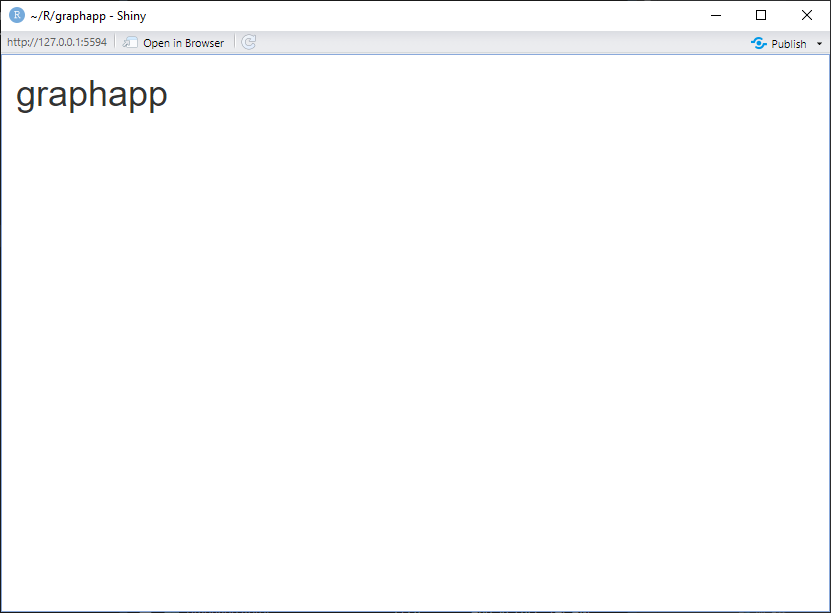
\includegraphics{/readme_img/shiny_01.png} \\
\midrule()
\endhead
Fig.1: The first run of the application. \\
\bottomrule()
\end{longtable}

You can create your own header using the basic \textbf{h1} tag along
with css on the UI side (\textbf{app\_ui.R}), e.g.,

\begin{verbatim}
app_ui <- function(request) {
    tagList(
        # code snippet...

        # Your application UI logic
        h1("Graph Simulator", style="background-color: #23b5fe;
                                     color: white;
                                     padding: 20px 15px;
                                     margin: 0;
                                     margin-bottom: 10px")
    )
}
\end{verbatim}

Given code is inserted in \textbf{app\_ui.R} file and results in a
differently styled header as seen in Fig.2.

\begin{longtable}[]{@{}l@{}}
\toprule()
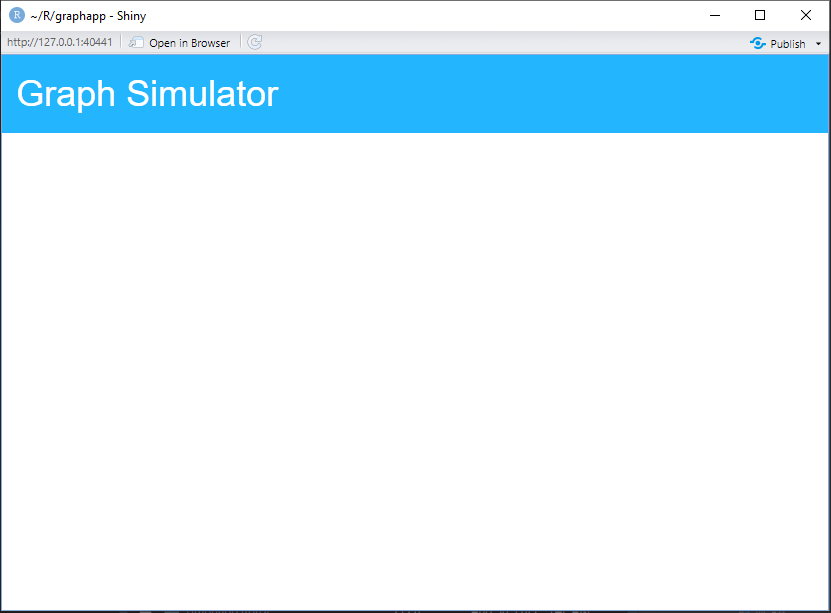
\includegraphics{/readme_img/shiny_02.png} \\
\midrule()
\endhead
Fig.2: Updated header. \\
\bottomrule()
\end{longtable}

\begin{verbatim}
To divide the application into "loading page" and "simulation page", you can use Shiny's tabsets layout.
\end{verbatim}

\begin{verbatim}
app_ui <- function(request) {
    # code snippet...

    fluidPage(
        tabsetPanel(
            tabPanel("Input",
                     h3("Load network graph")
            ),
            tabPanel("Simulation",
                     h3("Run the simulation")
            )
        )
    )
}
\end{verbatim}

The resulting layout is shown in Fig.3.

\begin{longtable}[]{@{}l@{}}
\toprule()
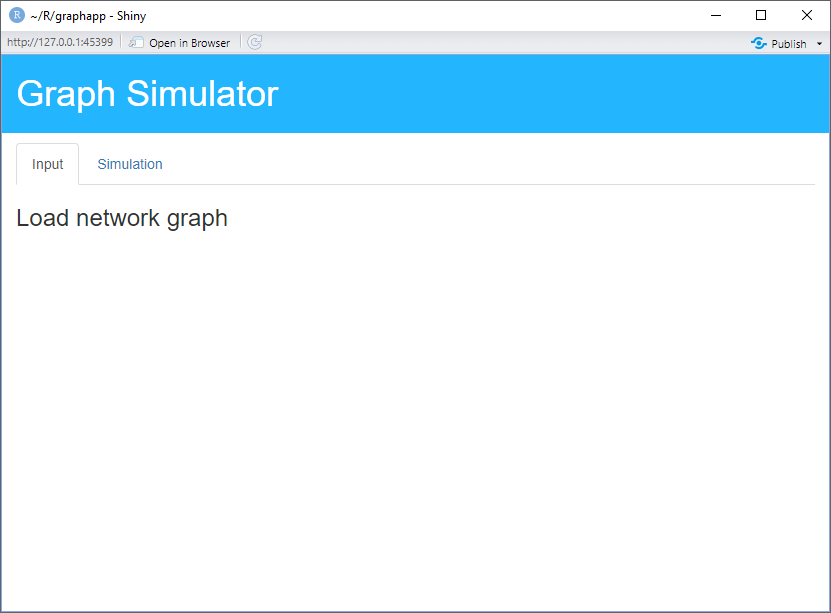
\includegraphics{/readme_img/shiny_03.png} \\
\midrule()
\endhead
Fig.3: Layout of the application. \\
\bottomrule()
\end{longtable}

Now, you need to put some logic in code to upload a csv file and
subsequently plot it. On the UI side, insert following lines of code in
the \textbf{tabsetPanel()}

\begin{verbatim}
tabPanel("Input",
         h3("Load network graph"),
         fileInput("upload", label = NULL),
         plotly::plotlyOutput("network")
)
\end{verbatim}

The \textbf{fileInput()} creates a button to open a file explorer. Once
the file is selected, it is sent to the server side under the id
\textbf{input\(upload**. The **plotlyOutput()** prepares the ground for the upcoming output from the server side under the id **output\)network}.
On the server side, i.e.~\textbf{app\_server.R}, the following needs to
be done.

\begin{verbatim}
app_server <- function(input, output, session) {
  # dataframe variable(s) ----
  r <- reactiveValues(
   df_network = NULL
  )

  # Upload network ----
  observeEvent(input$upload,
  {
      r$df_network <- utils::read.csv(input$upload$datapath,
                                      header = TRUE)
  })

  # Plotly ----
  output$network <- plotly::renderPlotly(
  {
    req(r$df_network)
    plot_network(r$df_network )
  })
}
\end{verbatim}

The data of the graph is prepared in a reactive way using
\textbf{reactiveValues()}. You can add as many variables as you need. In
this example, one variable
\textbf{r\(df_network** will be sufficient. Further, the **input\)upload}
is \textbf{NULL} when the app is launched. There is no data available,
yet. When its state is changed, it will trigger the
\textbf{observeEvent()}. An alternative is to use the \textbf{req()}
which ensures the following lines of code are triggered after some data
arrives (look into \textbf{renderPlotly()}). It blocks the \textbf{NULL}
state to proceed. Thus, when the data
(\textbf{r\(df_network**) is ready, they are sent to the **plot_network()** function. The output of the **plot_network()** represents data in a format suitable for the **plotlyOutput()** and they are stored in **output\)network}.
At the end of the process, the \textbf{output\$network} is used by
\textbf{plotlyOutput()} on the UI side. As the \textbf{plot\_network()}
is quite complex, the full code can be downloaded here
\href{https://github.com/It4innovations/NTS/blob/main/R/plot_network.R}{plot\_network()
code}. Feel free to browse through the given code.

An example CSV file can be downloaded
\href{https://code.it4i.cz/ADAS-Private/shiny-bpg/-/blob/main/inst/app/example_network.csv}{here}.
In short, the CSV file consists of 5 columns: \textbf{from},
\textbf{to}, \textbf{weight}, \textbf{level}, and \textbf{set}. Columns
\textbf{from} and \textbf{to} contain the name of nodes connected by a
single edge. The \textbf{weight} represents the weight of each edge. The
\textbf{level} holds the levels of each edge, i.e.~that the given edge
belongs to the set of ``the first floor'' (``the first row''), ``the
second floor'' (``the second row''), and so on. The \textbf{set}
represents the common sets of the edges within ``one floor'' (``one
row''). Different sets of one row will be drawed by different color. So,
after the \textbf{example\_network.csv} is uploaded into the app, the
graph of the network is plotted, see Fig.4.

\begin{longtable}[]{@{}l@{}}
\toprule()
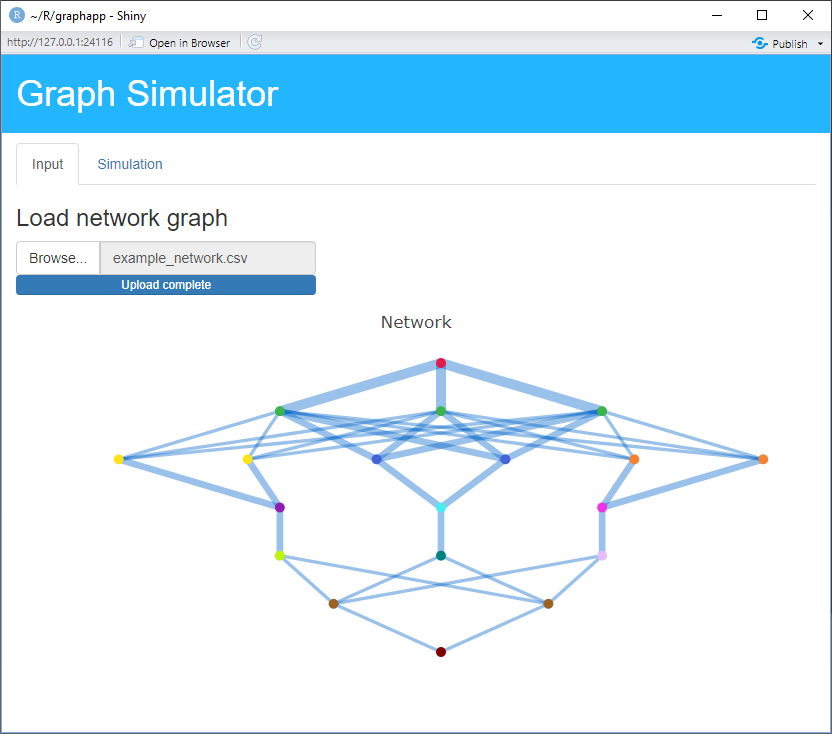
\includegraphics{/readme_img/shiny_04.png} \\
\midrule()
\endhead
Fig.4: Loaded graph. \\
\bottomrule()
\end{longtable}

At this moment, you have prepared the input data for the simulation.
Thus, the logic for the simulation along with the simulation function
has to be created. As it was said above, the input for the simulator is
the graph itself and the number of people that will go through the
graph. To do so, you can use the following code on the UI side into
\textbf{tabsetPanel()}.

\begin{verbatim}
tabPanel("Simulation",
    numericInput("input_people",
                 label = "Set the number of people that should enter the 
                          network.",
                 value = 100,
                 min = 10,
                 max = 5000,
                 step = 1
    ),
    textOutput("error_people"),
    actionButton("run",
                 label = "Compute simulation"
    ),
    h3("Simulation of the graph"),
    textOutput("error_graph"),
    plotly::plotlyOutput("simulation_plot")
)
\end{verbatim}

By the \textbf{numericInput()}, the number of people will be set. The
minimum number of people is set to 10 and the maximum to 5000. If the
number of people will be out of range, the error will be triggered on
server side and outputed into \textbf{textOutput(``error\_people'')}.
The \textbf{actionButton()} will start the simulation. The simulation
will be plotted by \textbf{plotlyOutput()}. Moreover, the
\textbf{textOutput(``error\_graph'')} will output an error message that
the button was clicked but there is no graph loaded.

The texts in \textbf{textOuput()} has black font as default. To change
it, you have to add \textbf{tags\(style** into **tags\)head} on the UI
side. Add \texttt{shinyjs::useShinyjs()}as well, it will be used later.

\begin{verbatim}
tags$head(
    # some code snippet...

    tags$style("#error_people, #error_graph { color: red; }"),
    shinyjs::useShinyjs()
)
\end{verbatim}

On the server side, prepare reactive values for the simulation.

\begin{verbatim}
app_server <- function(input, output, session) {
    # code snippet...

    # variables for simulation
    r_simulation <- reactiveValues(
        continue = NULL,
        simulation = NULL,
        animation = NULL
    )
}
\end{verbatim}

Then, observe if the \textbf{actionButton()} was clicked.

\begin{verbatim}
app_server <- function(input, output, session) {
    # code snippet...

    # observe if action button was clicked
    observeEvent(input$run,{
        r_simulation$continue <- NULL
        r_simulation$simulation <- NULL
        r_simulation$animation <- NULL
    
        shinyjs::disable("run")
    
        r_simulation$continue <- TRUE
    })
}
\end{verbatim}

As you can see, all the variables are reset after button was clicked.
The \texttt{shinyjs::disable("run")} disables the action button so you
will not be able to click on it until after the computation of the
simulation is done. The
\texttt{r\_simulation\$continue\ \textless{}-\ TRUE} tells the server
that the algorithm for the simulation can start. The simulation reads as
follows: If the
\textbf{r\_simulate\(continue** is **TRUE**, check if the **input\)input\_people}
is within the range. If not, output the error. If yes, check if the
network is loaded and there is an exit (sink) vertex in it. If something
is missing, output the error. If it is successful, compute the
simulation and store it into \textbf{r\_simulation\$simulate}.

The \textbf{check\_network()} function is part of the
\textbf{plot\_network()} code which was mentioned above. The
simulate\_flow() function is available here:
\href{https://github.com/It4innovations/NTS/blob/main/R/simulation.R}{simulate\_flow()}.
Do not forget to add \texttt{@import\ shinyjs} at the top of
\textbf{app\_server.R}.

\begin{verbatim}
app_server <- function(input, output, session) {
    # code snippet...

    # Simulation ----
    observeEvent(r_simulation$continue, 
    {        
        # Check input_people ----
        if (input$input_people > 5000 |
            input$input_people < 10)
        {
        
            # Output error if it is out of range
            output$error_people <- renderText("Input people should be 
                                               integer between 10 and 
                                               5000!")
            shinyjs::enable("run")
            input_people <- NULL
        } else {
            input_people <- round(input$input_people)
        }

        # Check network ----
        if (is.null(r$df_network)) 
        {        
            # output error if there is no graph loaded
            shinyjs::enable("run")
            output$error_graph <- renderText("The graph is not loaded!")
        } else {
            network_check <- TRUE
            if (check_network( r$df_network ) > 0)
            {
                network_check <- FALSE
                shinyjs::enable("run")
                output$error_graph <- renderText("The network definition  
                                                  is missing exit.")
            }
        }

        req(input_people, r$df_network, network_check)
        # if successful, reset error texts
        output$error_people <- renderText("")
        output$error_graph <- renderText("")
   
        res <- simulate_flow(df_edges = r$df_network, 
                             input_people = input_people)
        r_simulation$simulation <- res[[1]]
  })
}
\end{verbatim}

Finally, you have to output the animation. It can be done by following
code.

\begin{verbatim}
app_server <- function(input, output, session) {
    # code snippet...

    observeEvent(r_simulation$simulation,
    {
        print("Animating...")
        r_simulation$animation <-
            animate_simulation(df_edges = r$df_network,      
                               r_simulation$simulation)
    })

    observeEvent(r_simulation$animation,
    {
        output$simulation_plot <- plotly::renderPlotly(
        {
            r_simulation$animation
        })
        shinyjs::enable("run")
    })
}
\end{verbatim}

In other words, if the \textbf{r\_simulation\$simulation} is ready,
prepare the animation \textbf{by animate\_simulation()}, which can be
downloaded here
\href{https://github.com/It4innovations/NTS/blob/main/R/animate_simulation.R}{animate\_simulation()}.
If the animation is ready, output it by \textbf{plotly} and enable the
action button.

Congratulations, everything is ready to run the app. Type
\texttt{golem::run\_dev()} into the R console and try it yourself. The
app should look like as in Fig.5, below.

\begin{longtable}[]{@{}l@{}}
\toprule()
\includegraphics{/readme_img/shiny_run_final.gif} \\
\midrule()
\endhead
Fig.5: Example run of the application. \\
\bottomrule()
\end{longtable}

\hypertarget{adjustments-based-on-customers-review}{%
\subsection{Adjustments based on customers
review}\label{adjustments-based-on-customers-review}}

There was an update from the users that they want to add following
features:

\begin{itemize}
\tightlist
\item
  create and edit graph within the application,
\item
  export the graph into a csv file,
\item
  add special events that may occur in the simulation (e.g.~lunch
  break).
\end{itemize}

Such application already exists. You can try it yourself at
\url{https://shiny.vsb.cz/app/nts-shiny}. The source codes are available
here \href{https://github.com/It4innovations/NTS/}{NTS backend} and
\href{https://github.com/It4innovations/NTS_shiny/}{NTS Shiny}. It
extends the functionality of the app above. The \textbf{bs4dash}
features was used to easily style the app.

\newpage

\begin{center}

  
\includegraphics[width=0.3\textwidth]{media/image1.jpeg}

  \bigskip \bigskip \bigskip \bigskip \bigskip 

  
\includegraphics[width=0.35\textwidth]{media/image2.png}
  \qquad \qquad
  
\includegraphics[width=0.4\textwidth]{media/image3.png}

  \bigskip \bigskip \bigskip \bigskip \bigskip 

  
\includegraphics[width=0.4\textwidth]{media/image4.png}

  \bigskip \bigskip

This project has received funding from the European High-Performance Computing Joint Undertaking (JU) under grant agreement No 951732. The JU receives support from the European Union’s Horizon 2020 research and innovation programme and Germany, Bulgaria, Austria, Croatia, Cyprus, the Czech Republic, Denmark, Estonia, Finland, Greece, Hungary, Ireland, Italy, Lithuania, Latvia, Poland, Portugal, Romania, Slovenia, Spain, Sweden, the United Kingdom, France, the Netherlands, Belgium, Luxembourg, Slovakia, Norway, Switzerland, Turkey, the Republic of North Macedonia, Iceland, and Montenegro. This project has received funding from the Ministry of Education, Youth and Sports of the Czech Republic (ID:MC2101).

\end{center}

\end{document}
